\chapter{Background}
This thesis is based on several kinds of research of auto-tuning, evolutionary algorithms, and software optimization. This chapter summarizes the important aspects and details of approaches and optimization techniques used in the succeeding chapters.  

\section{Multi-Quality Auto-Tuning~(MQuAT)}

Multi-Quality Auto-Tuning (MQuAT) – is an approach to self-adaptive software, which provides design and operation principles for software systems that automatically provide the best possible utility to the user while producing the least possible cost.
It is based on the design-time part, which represents a new development method for self-optimizing systems and runtime parts, which concerns operation principles, namely,  novel techniques to runtime self-optimization~\cite{gotz13}.
MQuAT allows software developers to build and run software systems, which are automatically adjusted to provide the optimal user utility for the minimal cost. Such systems are comprised of multiple variants differing in their non-functional behavior and can analyze the reasons for the trade-offs between the respective non-functional properties (NFPs).  A key characteristic of MQuAT is the use of Quality of Service contracts to cover the inter-dependencies between NFPs,  the distinction between hard- and software, and the use of behavioral models to simulate complex non-functional behavior like \textit{energy consumption}.
In this thesis, MQuAT is used as a software environment that provides an optimization problem.


\section{MQuAT problem}

MQuAT problem was presented in ~\cite{gotz18}, and it consists of two problems:

\begin{itemize}
	\item Resource allocation in which the mapping of software component implementation to hardware resource leads to the least cost
	\item Variant selection, which provides the best utility by selecting better software implementations.
\end{itemize} 

To solve this problem was presented new generic metamodel. Both problems are interrelated by user requests specifying minimum requirements on the provided non-functional properties (i.e., minimum utility) while searching for a selection and mapping both to maximize utility and minimize costs. Correctness denotes that only solutions that \textit{do not violate} the users minimum requirements are considered \textbf{valid}.

The problem to be solved is selecting variants of software components and mapping them based on user requests to suitable hardware resources.

The MQuAT problem could be described as a metamodel which consists of:
\paragraph{Hardware metamodel}, which consists of hierarchically structured resource types and resources as instances of these types. So the hardware model composes static awareness of resources (types) and knowledge of runtime (instances). Certain types of resources can run the software, i.e., they are valid targets for software implementation mapping. The container attribute is used to mark such types. Figure~\ref{fig:HWmodel} depicted Hardware metamodel.

\begin{figure}
	\centering
	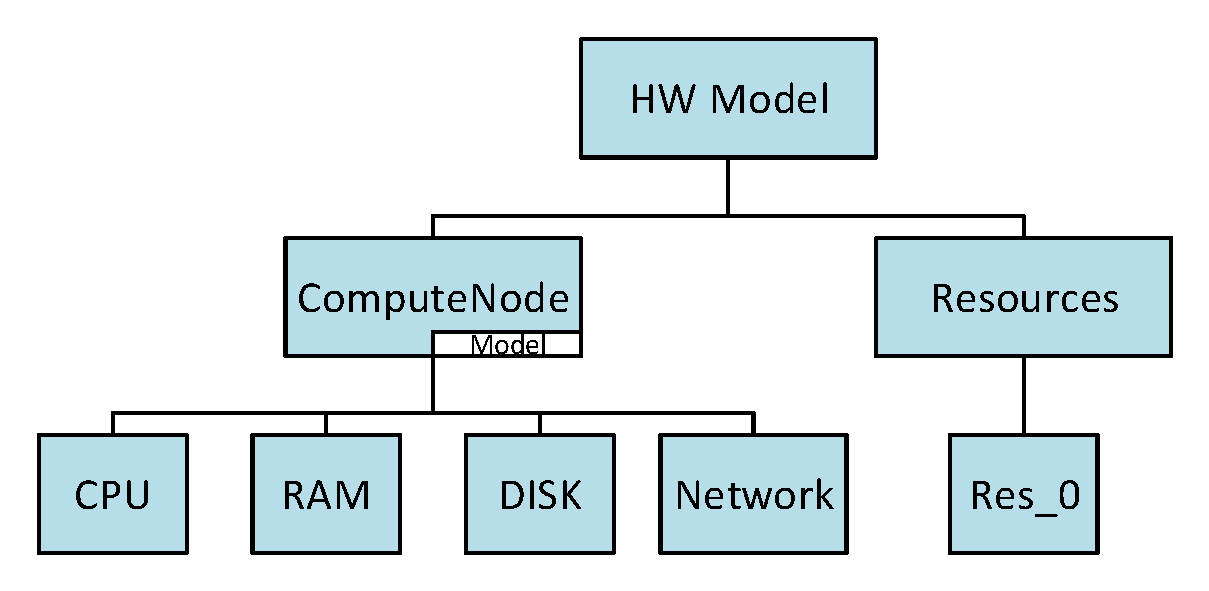
\includegraphics[width=0.8\textwidth]{images/HWModel}
	\caption[Hardware meta-model]{Hardware meta-model}
	\label{fig:HWmodel}
\end{figure}


In addition, a set of properties further characterize resource types. Resources specify then specific values for these properties. As an example, the resource type RAM could be defined with a property amount of memory and marked as a container.

\paragraph{Software metamodel} showed on Figure~\ref{fig:SWModel}. Its main element, called component and represents some functionality.
Each component consists of implementations that provide this functionality, requiring additional components or resources to complete their work. 

\begin{figure}
	\centering
	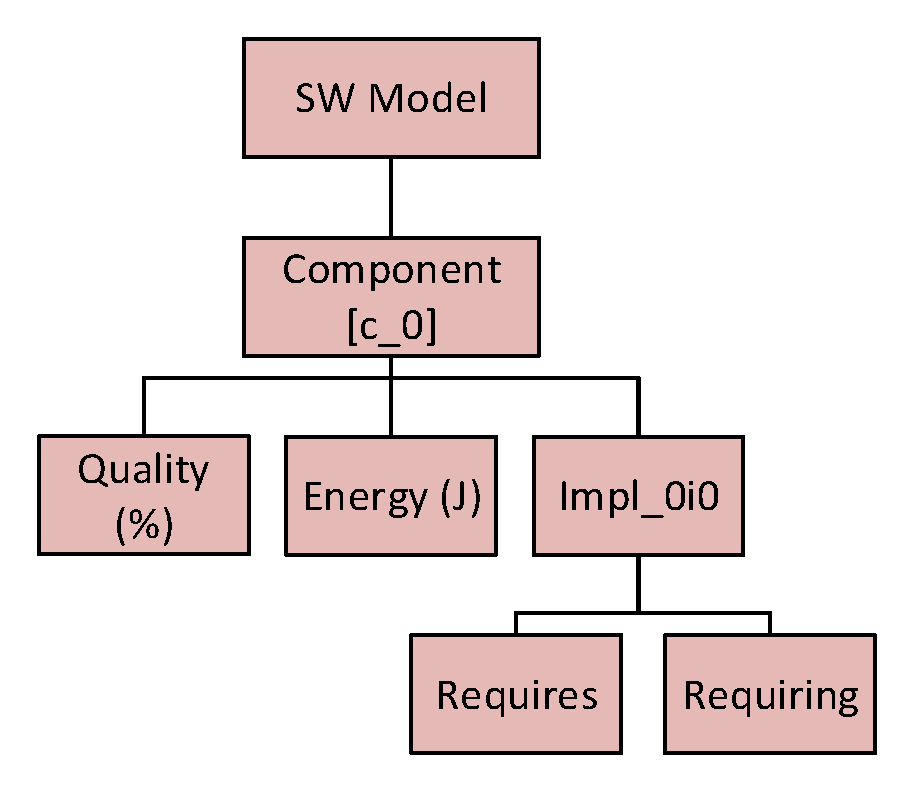
\includegraphics[width=0.5\textwidth]{images/SWModel}
	\caption[Software meta-model]{Software meta-model}
	\label{fig:SWModel}
\end{figure}

\paragraph{The Objective} specifies how to calculate a solution's objective value, i.e., for which value(s) the problem should be optimized. This selects a property to optimize for, and an objective function to define how to aggregate all values of this property.

\paragraph{A Request} represents a user requirement, which specifies which algorithm should be used to execute parameters and requirements. Requests contain their functional requirements by referring to a target software component, limitations on non-functional requirements (e.g., quality).\\

\paragraph
Full problem depicted on Figure~\ref{fig:mquatmodel}.

The problem description was changed in \cite{gotz2018JastAdd} and started to use the JastAdd framework\cite{ekman07} based on specified grammar. Aa a result, it gives a possibility of using reference attribute grammars~(RAGs)\cite{hedin2000} that adds computations in model nodes.
There are relations between component implementation and another software component that this implementation is requiring, between component implementation and HW resource that this implementation is required.


\begin{figure}
	\centering
	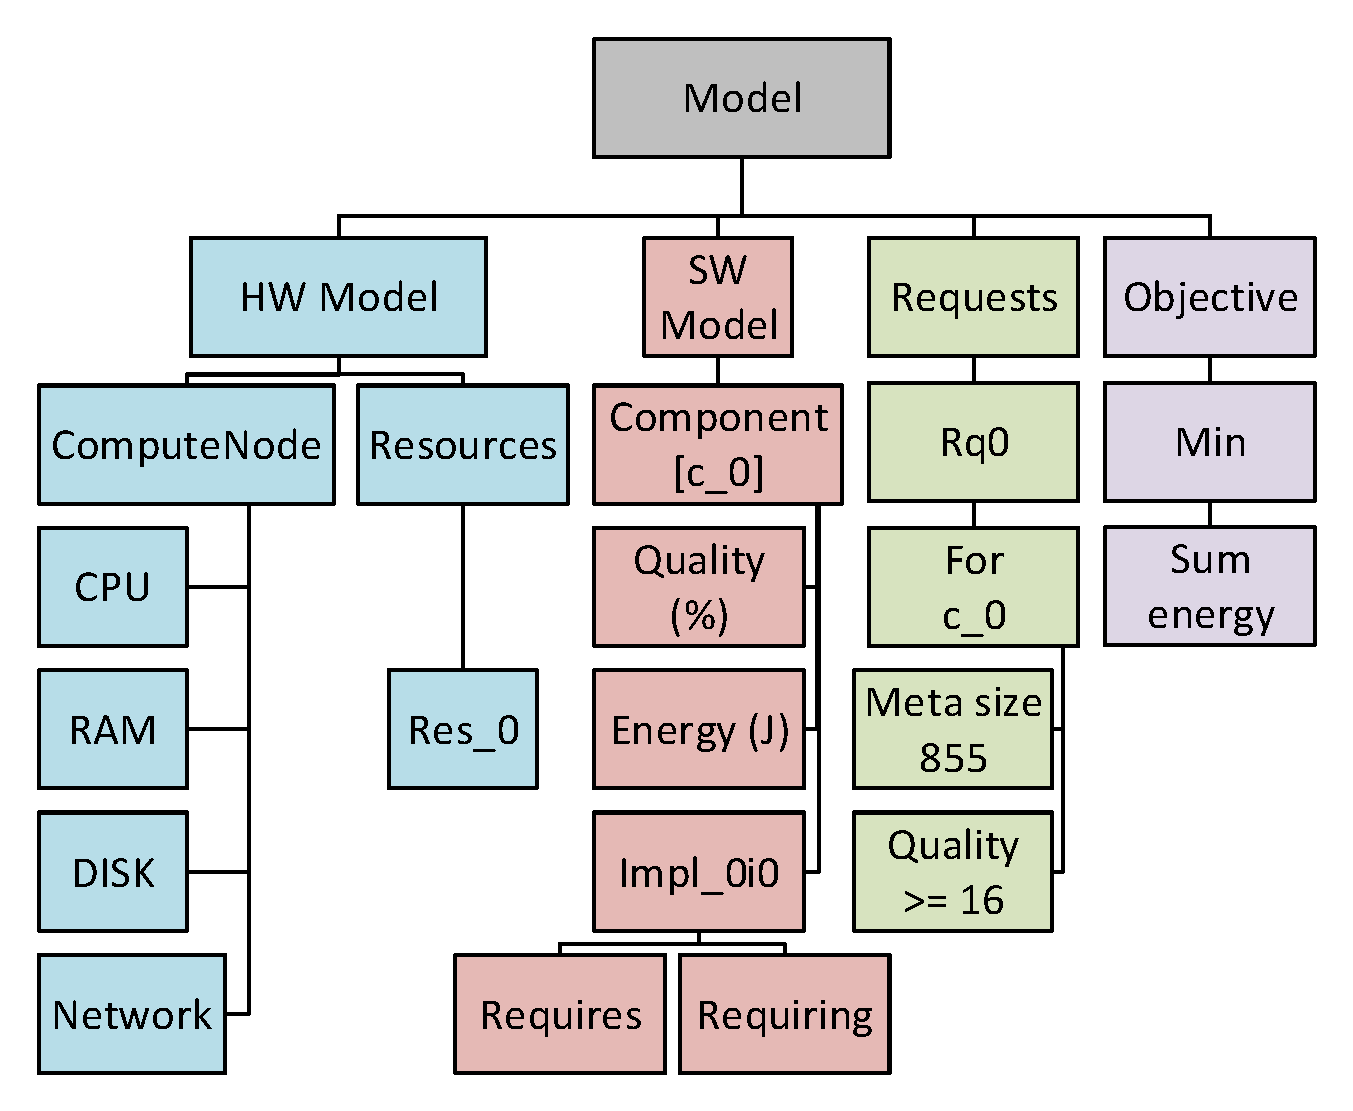
\includegraphics[width=\textwidth]{images/MQuATModel}
	\caption[MQuAT problem model]{MQuAT problem model}
	\label{fig:mquatmodel}
\end{figure}



There are some constraints that are grouped in Architectural, Request, and Negotiation constraints groups.

\begin{itemize}
	\item Architectural constraints ensure that each request is fulfilled, selecting exactly one implementation per component and deploying no more than one implementation on one resource.
	\item Request constraints ensure components are selected for each request so as to provide the requested non-functional properties.
	\item Negotiation constraints ensure non-functional requirements are met depending on the implementation.
\end{itemize}

There are additional constraints due to problem generation:

\begin{itemize}
	\item structures for the software and hardware components are fixed to ensure comparability,
	\item \texttt{computeNode} that represents a regular computer hardware consist of one or more CPUs, RAM memory, disk, and a networking interface,
	\item software model has a simple tree structure,
	\item fixed branching factor of two.
\end{itemize}

Each MQuAT problem is characterized by four parameters:

\begin{itemize}
	\item[Software variants] - the number of implementations for each software component,
	\item[Number of requests] - the number of requests to run software components, that described by user, 
	\item[Component tree depth] - the depth of the software tree, that describes the dependency of software components,
	\item[Resources ratio] - this parameter describes the number of available hardware resources. The number of HW resources calculated as the multiplication of the number of nodes of the component tree by the number of requests and multiplied by the resource ratio.
\end{itemize}

\section{The solution of the MQuAT problem}

The solution is computed by the MQuAT solver. There are many solvers:

\begin{itemize}
	\item Simple solver, which goes step by step from one solution candidate to another.
	\item ILP solver, which generates integer linear programming (ILP) problem from the MQUAT problem and after that solve it.
	\item Random solver - tries random solution candidates.
	\item Simulated Annealing (SA) solver, based on the simulated annealing meta-heuristic~{pukhkaiev19}.
	\item Genetic solver that uses a genetic algorithm to solve the problem.
\end{itemize}

In this thesis, we talk about Genetic solver in detail in the next sections.
The solution could be represented as a tree structure. An example of the solution shown in Figure ~\ref{fig:SolutionModel}

It contains a list of assignments. Each assignment selects one implementation of the required component and maps it to the resources~\cite{gotz18}.
A solution is valid if for each user request.

\begin{enumerate}
	\item an implementation is deployed for the target component,
	\item for each component required implementation is deployed,
	\item all necessary (non-functional) property clauses (including request constraints) are met,
	\item at most one implementation for each resource is deployed.
\end{enumerate}

If it is valid and no other solution has a better objective value, then a solution is optimal~\cite{gotz18}.

\section{Evolutionary algorithms}
\label{sec:GeneticAlgorithm}

Evolutionary algorithms are a subset of evolutionary computation and belong to set of modern heuristics-based search method.~\cite{vikhar16}
This domain contains different variants, such as:
	\paragraph{Genetic algorithm~(GA)} - is the most widely known type of EA\cite{eiben03}. The research~\cite{deJong75} presented the description of the simple GA, that has a binary representation~(bit strings), proportional selection and a low probability of mutation. Has a fixed flow. The entire population changes on each generation. On the current moment, more preferable to use the rank-based selection, one point crossover changed to the alternatives. And most important, that developers use not binary representation that increase an understanding of the problem that GA solving.
	\paragraph{Evolution strategy~(ES)} - that works with vectors representation of a solution. New offspring is generated by adding random values to the elements in the vector. Use self-adaptation for own parameters. ES self-adapt  the mutation step sizes.
	\paragraph{Evolutionary programming~(EP)} - was developed with the aim to get artificial intelligence\cite{eiben03}. Has the same representation as ES, but do not use the recombination. The selector algorithm selects parents from the union of the population and new offspring.
	\paragraph{Genetic programming~(GP)} - use as a representation of chromosomes a tree shaped structures. Recombination works by sub-tree exchanging. A particular difference is the work flow. A GP performs either a crossover or a mutation, and a GA performs two operations in sequence.

\begin{figure}
	\centering
	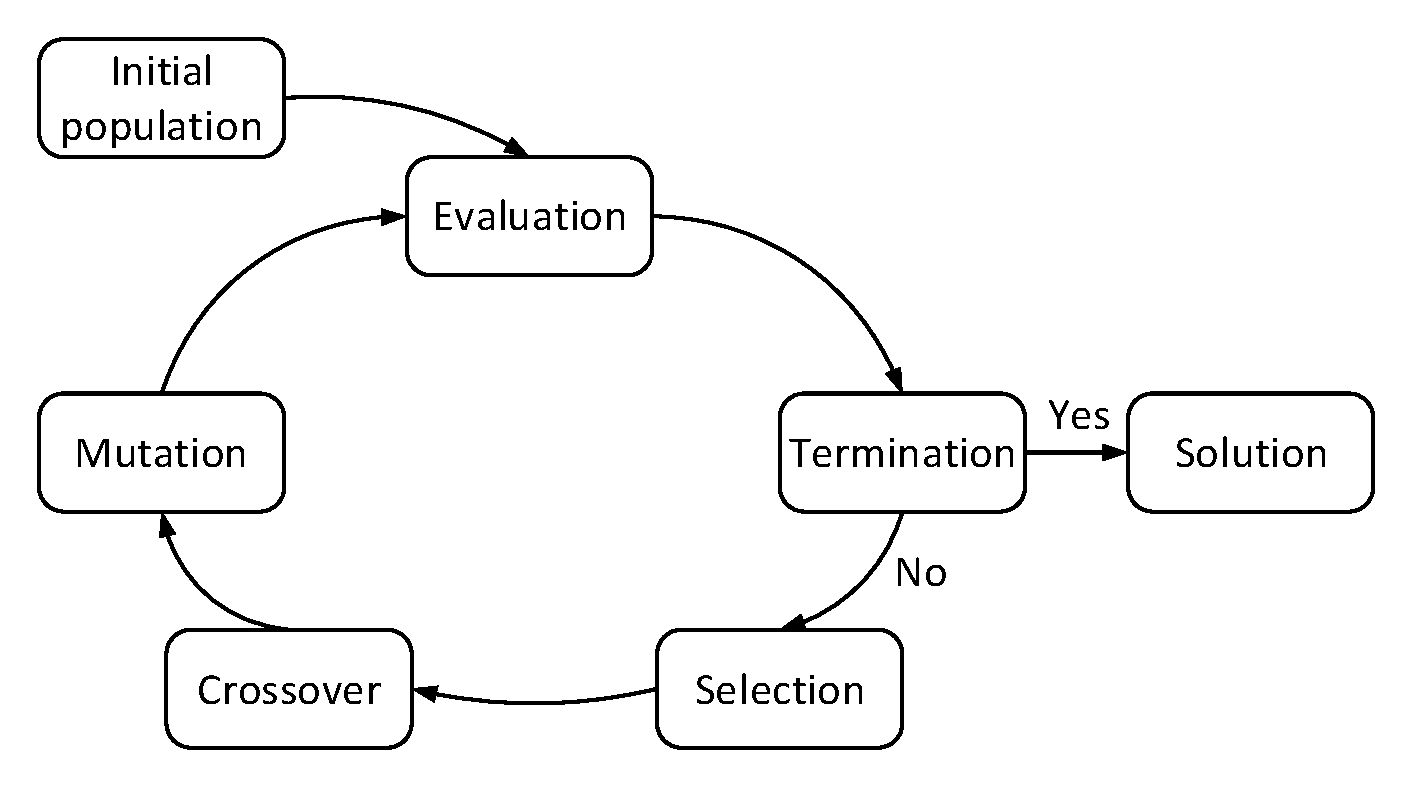
\includegraphics[width=0.8\textwidth]{images/GeneticLoop}
	\caption[Main loop of the genetic algorithm]{Main loop of the genetic algorithm}
	\label{fig:GeneticLoop}
\end{figure}

The main principle of EA looks like a loop with several steps.
The first step is the creation of an initial population - a set of randomly created individuals; each of them represents one solution. 
The second step is Evaluation. Calculate the fitness or objective function of the current population.
If the solution is founded and all requirements for the termination are fulfilled, then we get the final solution. Otherwise, select the best candidates to create a new generation.
In step 4, using recombination and mutation on selected candidates, GA creates a new generation of the population. And after that, evaluate it.

GA is based on different components and operators.

\subsection{Selector}\label{sec:GeneticAlgorithm:Selector}

The selector is one of the most important components of the EA. It selects \textit{\textbf{mu}} number of individuals from the population, that used to create new \textit{\textbf{lambda}} number of individuals. There are many different selection algorithms.


	\paragraph{NSGA-II~(Non-dominated sorting based genetic algorithm)~\cite{deb2000}} - is a multi-objective selection algorithm. It searching for noon-dominated solutions. Figure~\ref{fig:nsga2} demonstrates how it works. There is a population \texorpdfstring{R\textsubscript{t}}{R t} that consist of two sets. First set is a parent population. It marked as \texorpdfstring{P\textsubscript{t}}{P t}. The second set is new offspring and marked as \texorpdfstring{Q\textsubscript{t}}{Q t}. Combined population \texorpdfstring{R\textsubscript{t}}{R t} is sorted using non-dominated sorting. After that it generate a Pareto front. After sorting, selector selects the new population \texorpdfstring{P\textsubscript{t+1}}{P t+1} of size represented as a parameter by binary tournament selection and use it for the next round of reproduction.
	
	\begin{figure}
		\centering
		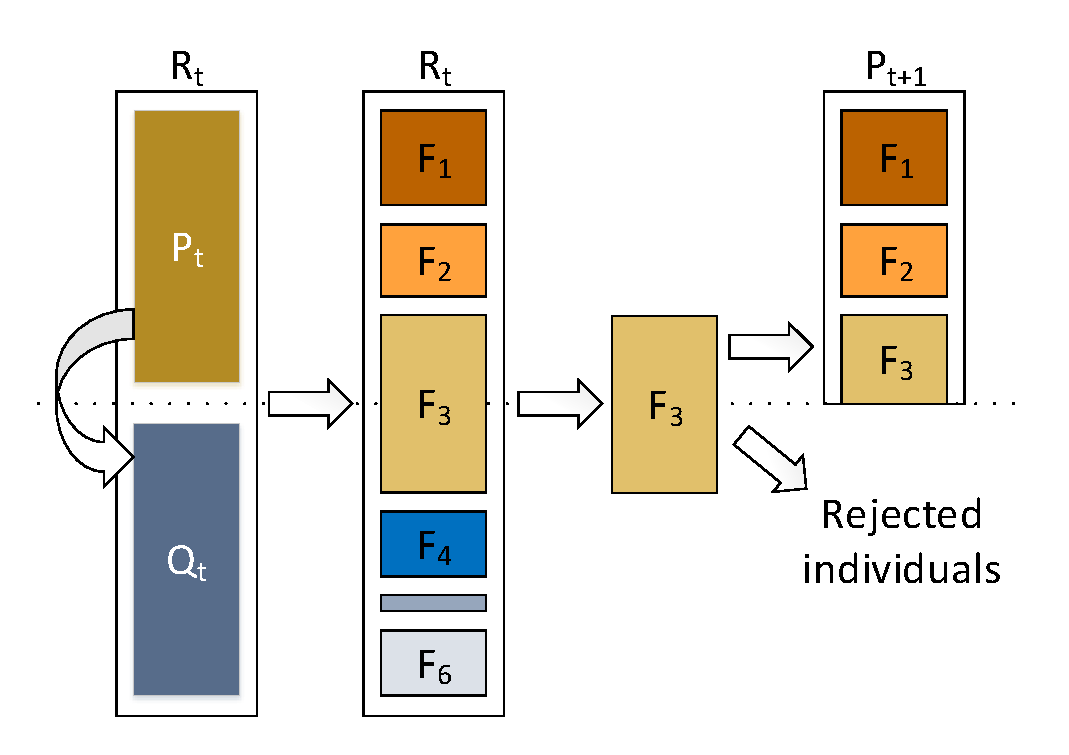
\includegraphics[width=0.75\textwidth]{images/nsga2.pdf}
		\caption[NSGA-II]{NSGA-II}
		\label{fig:nsga2}
	\end{figure}
	
	\paragraph{SPEA2~(Strength Pareto Evolutionary Algorithm)~\cite{zitzler01}} - a multi-objective selection algorithm, that used to find the Pareto optimal solution for multi-objective problems\cite{zhihuan2010}. Figure~\ref{fig:spea2} demonstrate how it works.
	There are two sets. First one is a current population that marked as \texorpdfstring{R\textsubscript{t}}{R t}. The second is an archive set. It marked as \texorpdfstring{A\textsubscript{t}}{A t}. SPEA2 takes the union of all solutions in \texorpdfstring{R\textsubscript{t}}{R t} and in \texorpdfstring{A\textsubscript{t}}{A t}. The union set marked as \texorpdfstring{U\textsubscript{t}}{U t}. After that it compares the size of \texorpdfstring{U\textsubscript{t}}{U t} and archive size. If \texorpdfstring{U\textsubscript{t}}{U t} is grater than archive size then SPEA2 reduce the union population. If \texorpdfstring{U\textsubscript{t}}{U t} is less  size then SPEA2 extend the population from the dominated solutions. After that, it selects best non-dominated solutions that used in next iteration.
	
	\begin{figure}
		\centering
		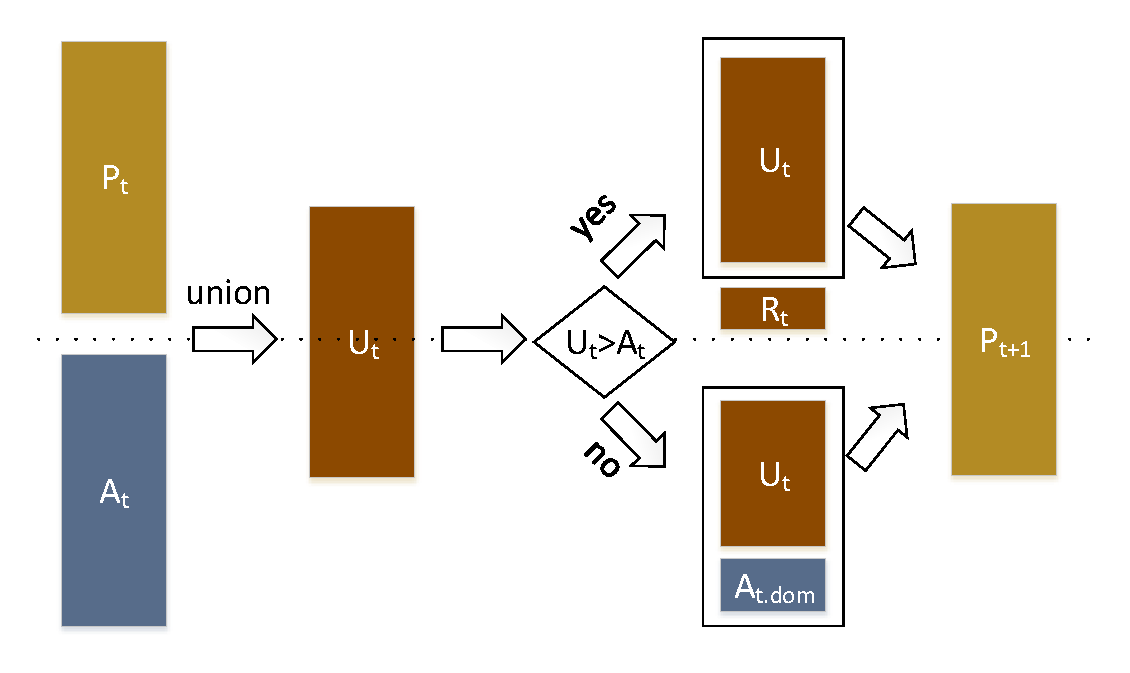
\includegraphics[width=0.9\textwidth]{images/spea2Selector.pdf}
		\caption[SPEA2]{SPEA2}
		\label{fig:spea2}
	\end{figure}
	
	\paragraph{NSGA3~\cite{deb14}} - it extends NSGA-II to using references points to handle multi-objective problems and its usage on one- or two-objective problems is discouraged.
	\paragraph{SPEA3} - presented in~\cite{rudzinski15}. It is a generalization of SPEA2 that consists in the exchange of the selection procedure that aims to determine the the non-dominated solutions with a high spread and balanced distribution. Aa described by researches, it works well with two- and three-objective problems. //

In this thesis, we focus on a selection algorithm only as a parameter of a genetic algorithm and use NSGA-II and SPEA2 due to software constraints of the used framework. 

\subsection{crossover}\label{sec:GeneticAlgorithmCrossover}

Crossover is an operator of a genetic algorithm that allows the recombination of two individuals by swapping some genes between them.
In general, the crossover has several parameters such as

\begin{itemize}
	\item Crossover rate - parameter that describes the probability of two chromosomes to exchange their genes.
	\item Crossover point - the point in which the exchange could be done.
\end{itemize}

The principle of the crossover is next.
Firstly, select the crossover point. For example, a chromosome could be described as a vector of bits. Then the crossover point is the start index of bits, which were replaced by another chromosome.
Secondly, it swaps genes between chromosomes.

\begin{figure}
	\centering
	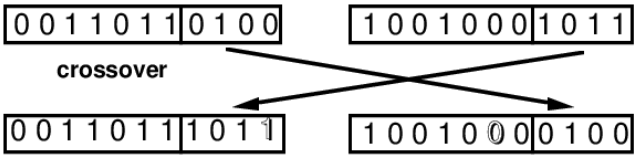
\includegraphics[width=0.5\textwidth]{images/crossoverVector.png}
	\caption[Example of the crossover]{Example of the crossover between chromosome that described as a vector of bits}
	\label{fig:crossoverVector}
\end{figure}

\subsection{mutation}\label{sec:GeneticAlgorithmMutation}

The mutation is an operator of a genetic algorithm that changes a single gene in a chromosome. As a crossover operator, a mutation has parameters:

\begin{itemize}
	\item Mutation rate - parameter that describes the probability of mutation.
\end{itemize}

To perform a mutation on chromosome need to do:

\begin{enumerate}
	\item Randomly select gene which mutates
	\item Change selected gene to another.
\end{enumerate}

\begin{figure}
	\centering
	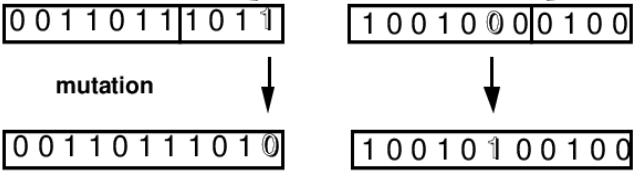
\includegraphics[width=0.5\textwidth]{images/MutationVector.png}
	\caption[Example of the mutation]{Example of the mutation between chromosome that described as a vector of bits}
	\label{fig:MutationVector}
\end{figure}

Figure~\ref{fig:MutationVector} presented a simple mutation on the chromosome that described as a vector of bits.




\section{Genetic solver}\label{sec:GeneticSolver}
The genetic solver was created to solve the MQuAT problem. It was developed by Jamal Ahmad in ~\cite{ahmad18}. And further improved by Johannes Mey.

This solver is based on Opt4J framework~\footnote{http://opt4j.sourceforge.net/download.html}. It's an open-source framework that gives the opportunity to implement a genetic algorithm for custom optimization problem by specifying several modules and classes.

To solve the custom problem using genetic algorithm, the user needs to create several things:

\begin{enumerate}
	\item Creator is needed to create a random genotype for the initial population.
	In the genetic solver Creator create the genotype by creating a random solution model and transform it into a Tree Shape Genotype structure.
	\item Decoder is needed to perform decoding the tree shape genotype into phenotype. The phenotype, in this case, is a Solution Model of MQuAT.
	\item Evaluator calculates the objective functions of the solution. In the case of genetic solver, the Evaluator calculates two objectives: 
	
	\begin{itemize}
		\item Validity errors - number of violated contracts
		\item Energy value - energy consumption
	\end{itemize}
	
\end{enumerate}

If your genotype can't be described as a vector, then you first need to implement:

\begin{enumerate}
	\item Genotype
	\item Crossover operator
	\item Mutation operator
\end{enumerate}

\subsection{Tree Shape Genotype}

Because of the problem model of MQuAT, which requires mapping of implementations to resources, in genetic solver was created Tree Shape Genotype~\cite{ahmad18}.
The example of this genotype shown on Figure~\ref{fig:TreeShapeGenotypeExample}

\begin{figure}
	\centering
	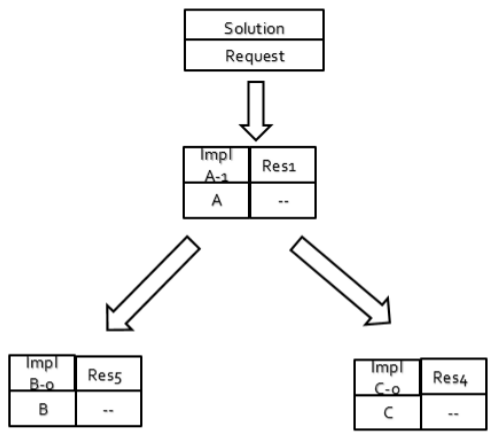
\includegraphics[width=0.6\textwidth]{images/TreeShapeGenotypeExample.png}
	\caption[Example of the Tree Shape Genotype]{Example of the Tree Shape Genotype}
	\label{fig:TreeShapeGenotypeExample}
\end{figure}

The first node in this genotype contains the input request. The second node represents the mapping of the user component. In this node, Impl A-1 is selected rather than Impl A-0 of the user component. As shown in Figure~\ref{fig:TreeShapeGenotypeExample}, this implementation is mapped to Hardware-Resources1. Moreover, Impl A-1 also requires software components B and C that have only one Impl B-0 and Impl C-0 implementation and are mapped to Hardware-Resource5 and Hardware-Resource4, respectively.

\subsection{Crossover operator}
\label{sec:GeneticSolverCrossover}

This operator performs a crossover between two Tree Shaped Genotypes and are performed on software implementation and hardware resource in each tree shape genotype. 
Crossover process starts on the root of the both tree. Crossover operator compare if the implementation and mapped resource of both nodes are same. If not the same, then with probability described as a parameter \texttt{CrossoverProbability} it swaps the implementations, resources and lower substructure of the tree. It swaps the subtree in order to maintain the consistency. If comparison says that nodes are identical, then it performs the crossover process for each child node. Such recursive algorithm gives a possibility to perform the crossover on a few points of the Tree Shape Genotype as it showed in Figure~\ref{label}. Crossover points have a gray color.

\begin{figure}
	\centering
	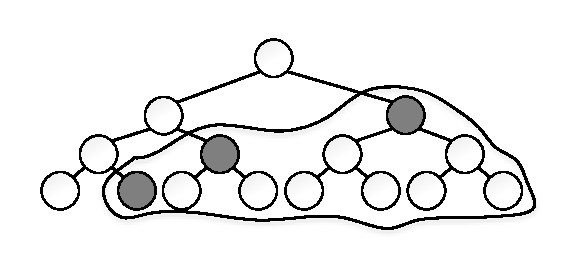
\includegraphics[width=\textwidth]{images/CrossoverPoints.pdf}
	\caption[Crossover Points]{Crossover Points}
	\label{fig:CrossoverPoints}
\end{figure}

Figure~\ref{fig:GeneticSolverCrossover} depicted the crossover between two genotypes. Each genotype has 3 nodes. The Crossover starts on root nodes. These nodes have the same implementation and resource. As a result, crossover recursively goes down to children. As showed, first child of both genotypes have different implementation and resource and crossover swap them with the probability \texttt{CrossoverProbability}. After that crossover operator performs comparison for the second child.


\begin{figure}
	\centering
	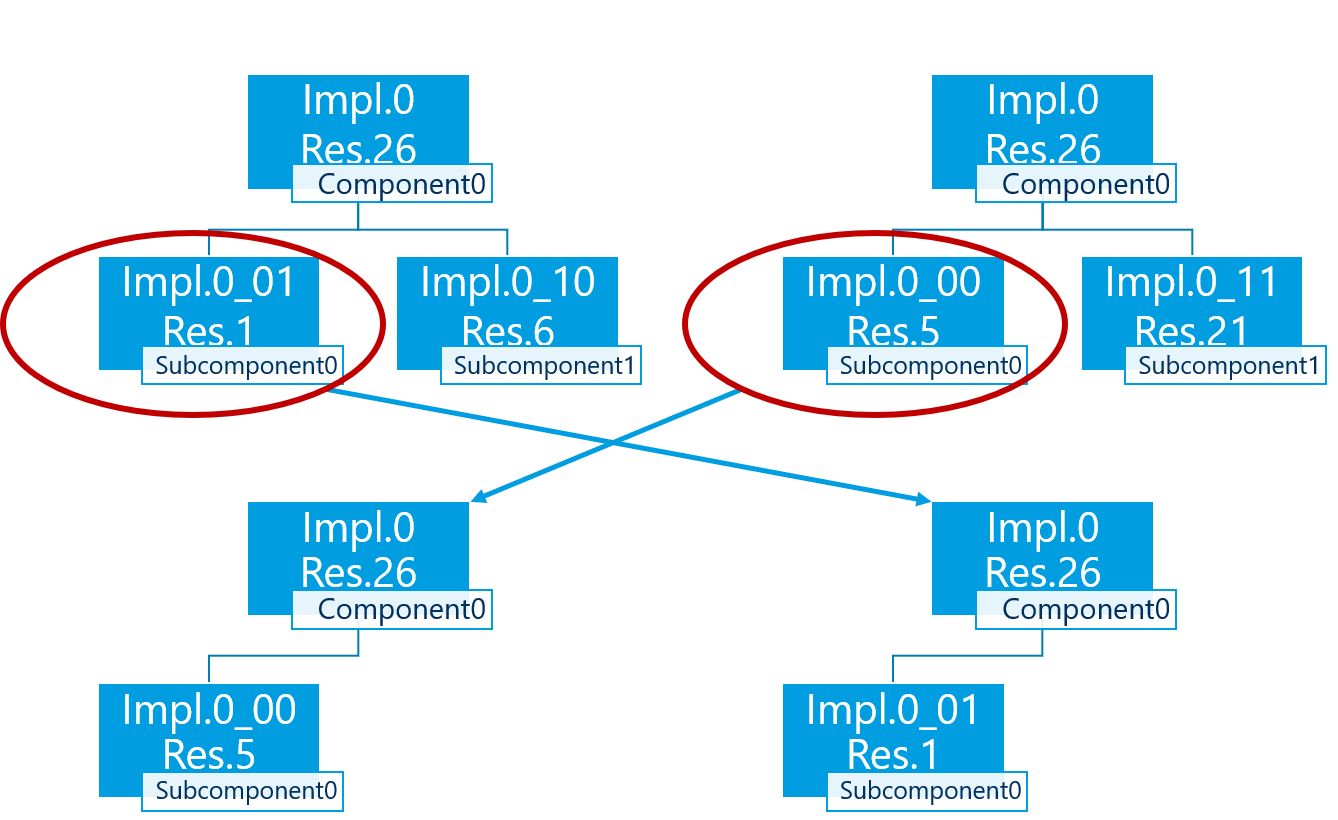
\includegraphics[width=0.9\textwidth]{images/GeneticSolverCrossover.png}
	\caption[Crossover in Tree Shape Genotype]{Example of crossover between two Tree Shape Genotypes}
	\label{fig:GeneticSolverCrossover}
\end{figure}



\subsection{Mutation operator}
\label{sec:GeneticSolverMutation}
Mutation operation is used to randomly add new features to the tree-shaped genotype.
Mutation occurs for one random request. With some probability that described by parameter \texttt{MutationRate} it mutate the root node. If mutation operator mutate the top node of the tree, there is a probability to mutate tre resource. This probability described with parameter \texttt{ResourceMutationProbability}. Or it will mutate the implementation of the top node. And change lower structure for consistency. If mutation will occur not in the root of the genotype, then the process recursively goes down to children.  Figure~\ref{fig:GeneticSolverMutation} depicts the mutation process in which mutation was performed on the resource 
in the root node.

\begin{figure}
	\centering
	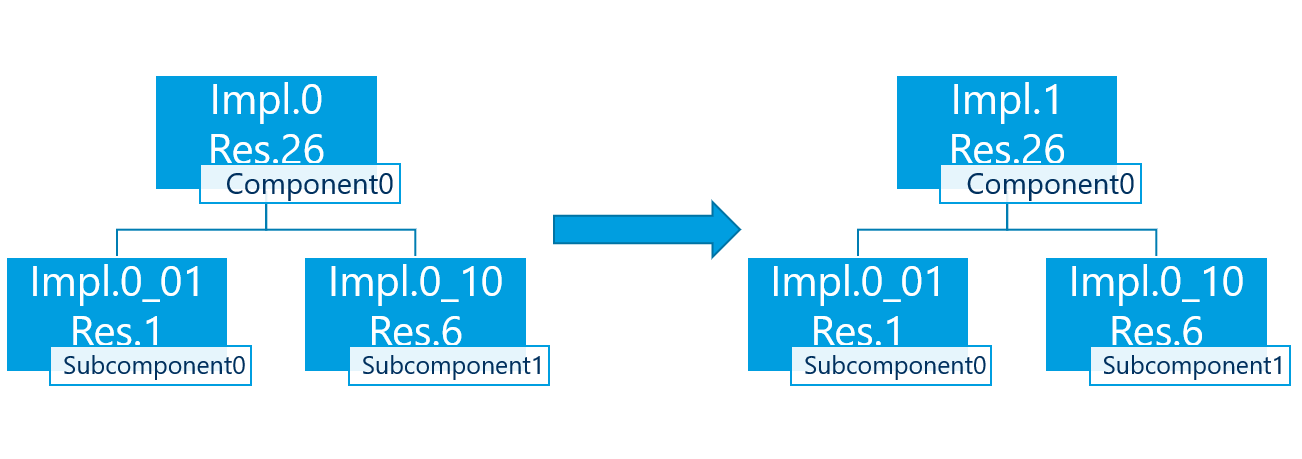
\includegraphics[width=\textwidth]{images/GeneticSolverMutation.png}
	\caption[Mutation in Tree Shape Genotype]{Example of mutation between two Tree Shape Genotypes}
	\label{fig:GeneticSolverMutation}
\end{figure}

\section{Parameter Tuning Strategies for GA}\label{sec:Parameter Tuning Strategies}

information from literature!\todo{will add more in next draft}

\section{BRISE}\label{sec:BRISE}

BRISE is a software product line (SPL) for parameter tuning~\cite{pukhkaiev19}.
This SPL has two conceptual parts:

\begin{itemize}
	\item Static part describes the main flow of parameter tuning, task management, and reporting.
	\item Configurable parts should be configured for each experiment.
\end{itemize}

\begin{figure}
	\centering
	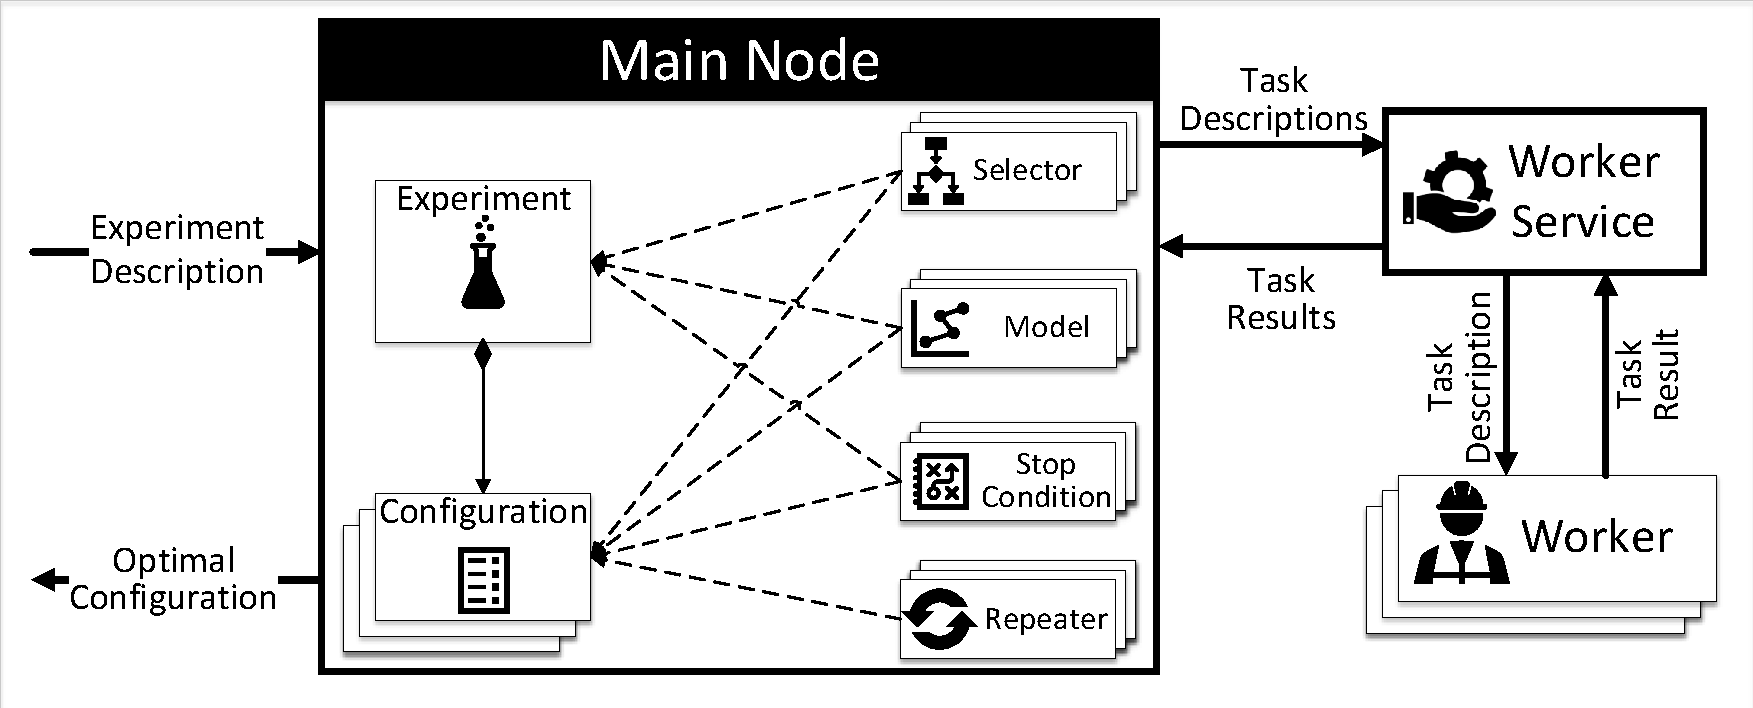
\includegraphics[width=\textwidth]{images/BRISEarch.pdf}
	\caption[The high-level architecture of BRISE]{The high-level architecture of BRISE}
	\label{fig:BRISEarch}
\end{figure}

Figure~\ref{fig:BRISEarch} shown the high-level architecture of BRISE.
Configurable part consists of 
\paragraph{Experiment description} - describes the experiment, parameters that need to tune, the objective of the experiment, and expected values to detect outliers.
\paragraph{Selector} - selection algorithm that is used to get the combination of parameters from the search space of all possible combinations. BRISE has two selection algorithms out of the box: Sobol sampling~\cite{sobol99} and Fedorov's exchange algorithm~\cite{fedorov13}. 
\paragraph{Model} - predict new configuration. New Model builds after each iteration of measurement of configuration, and if the model predicts a valid result, this configuration goes to be measured in the next iteration. BRISE has several models out of the box.
\paragraph{Stop condition} - the component that analyzes the results of the experiment, validates the result, and makes a decision to stop the experiment or continue. There are many different stop conditions that could work as a combination of criteria.
\paragraph{Repeater} - component of BRISE that decide about the number of measurement for each configuration to get need accuracy of the results. 
\paragraph{Worker} - contains the process that BRISE needs to tune. Run this process with different configurations and returns the metric of this configuration to use it in the next model build.
All components from the configurable part could be extended by users to achieve their goals.

BRISE has two modes: \textit{Search space exploration} and \textit{Hyperparameter tuning}.
The first mode is used to get information about the search space of hyperparameters. In this mode, there are no predictions cause BRISE uses the selector to cover the search space. As a result of using BRISE without predictions, the model component is disabled.

The second mode is used to find the optimized values for hyperparameters. All components of the main node are used in this mode.

The main principle of how BRISE works in both modes is the same, but 
Search space exploration mode has one exception.

The user prepares a target system that will be running in workers and measure the result for the specified configuration of hyperparameters.
After that user describes the experiment description - JSON file that contains all information about hyperparameters, their ranges and default values, result structure, expected ranges for result values, and the max time needed to run one task.

The user input of BRISE is an experiment description that in BRISE transforms into the experiment object after that BRISE starts working.

It starts with the measurement of the default configuration. When the default configuration had been measured, the selector gives a set of new configurations to be measured. After measurements, workers return the results to the main node. The repeater checks the result and decides to measure this configuration one more time, or results have needed accuracy. 

On the next step model component tries to build the model and validate itself. If a model is valid, then it predicts a new configuration. If the model is not valid, BRISE gets a new configuration from the selector. BRISE sends it to worker service to measure and get the result. If SPL is working in Search space exploration mode, the model build step is skipped, and new configuration always received from the selector. 

These measurements are performing until stop condition criteria in stop condition components are met.
